\begin{figure}[ht!]
    \centering
    % \begin{tabular}[c]{ccc}
    % \begin{subfigure}[c]{0.31\textwidth}
    %     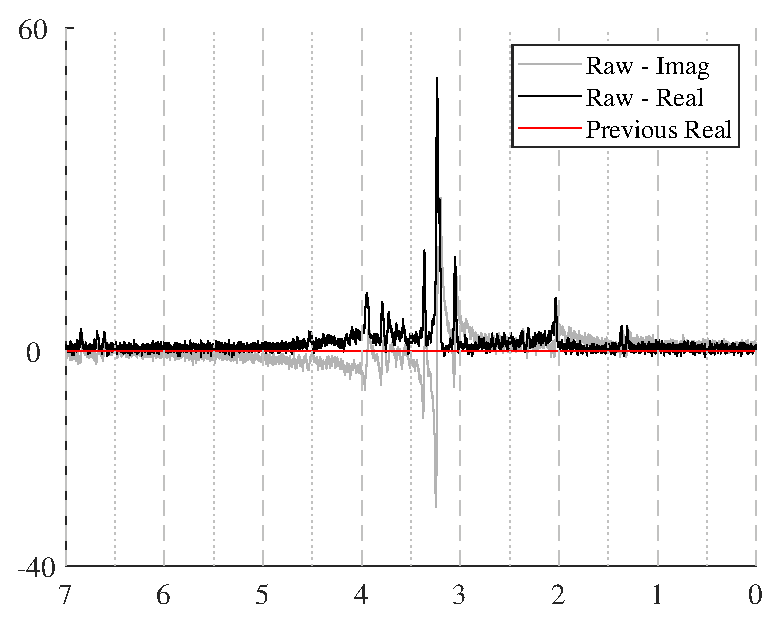
\includegraphics[width=0.93\textwidth,keepaspectratio]{images/30ms_B0_samples/30ms_curated_B0_sample_1Hz.eps}
    %     \vspace{3pt}
    % \end{subfigure}&
    % \begin{subfigure}[c]{0.31\textwidth}
    %     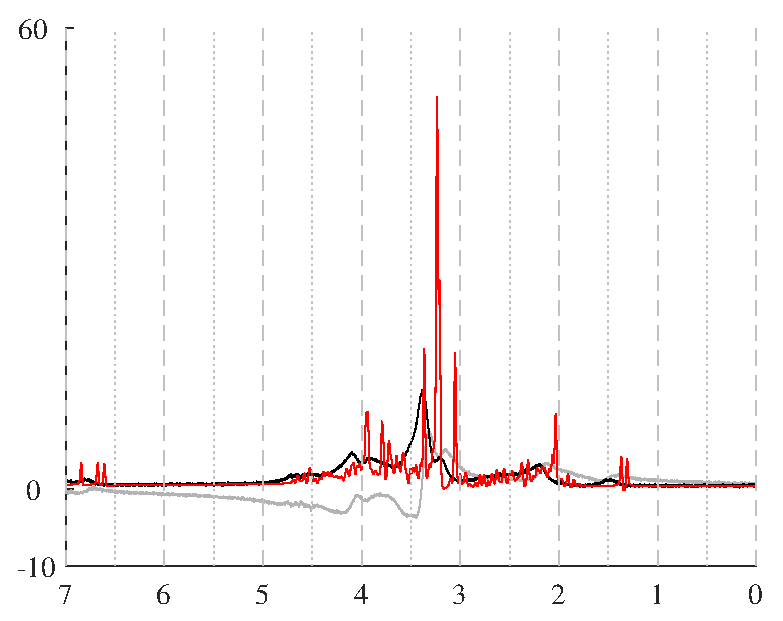
\includegraphics[width=0.93\textwidth,keepaspectratio]{images/30ms_B0_samples/30ms_curated_B0_sample_20Hz.eps}
    %     \vspace{3pt}
    % \end{subfigure}&
    % \begin{subfigure}[c]{0.31\textwidth}
    %     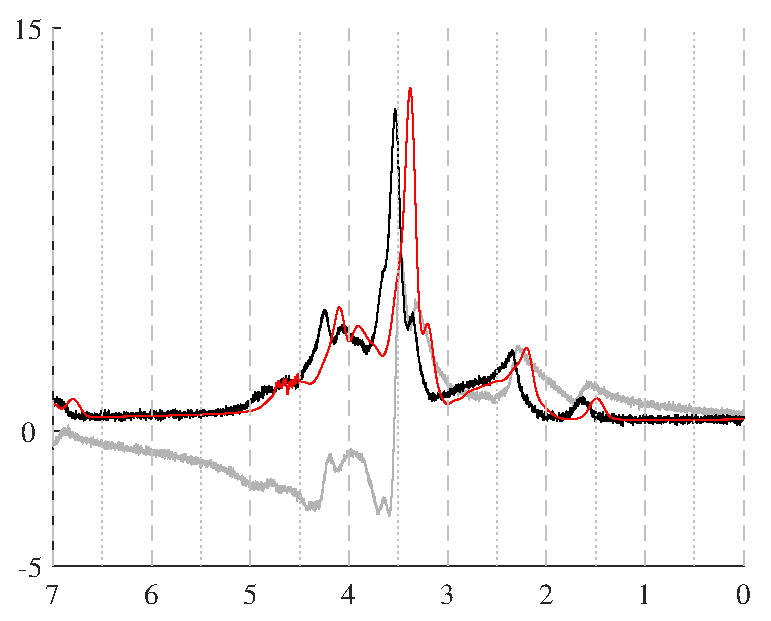
\includegraphics[width=0.93\textwidth,keepaspectratio]{images/30ms_B0_samples/30ms_curated_B0_sample_39Hz.eps}
    %     \vspace{3pt}
    % \end{subfigure}\\
    % \begin{subfigure}[c]{0.31\textwidth}
    %     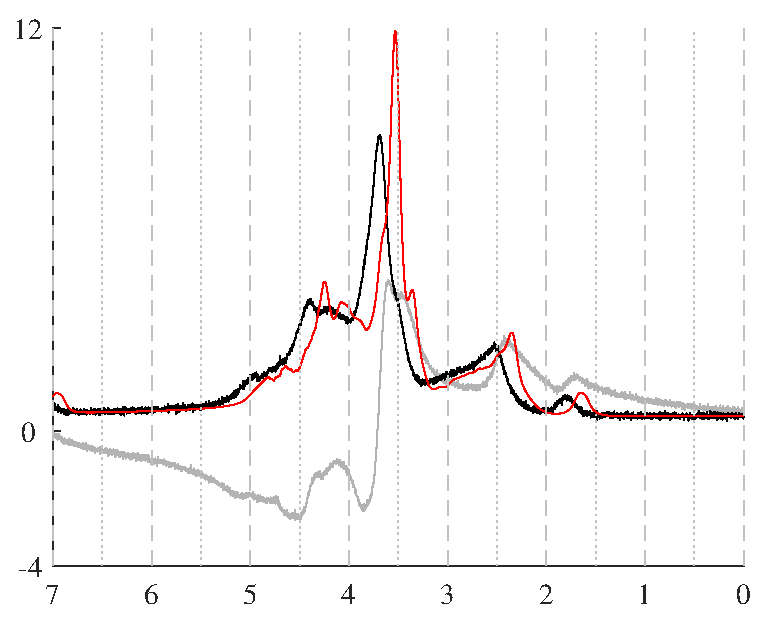
\includegraphics[width=0.93\textwidth,keepaspectratio]{images/30ms_B0_samples/30ms_curated_B0_sample_59Hz.eps}
    %     \vspace{3pt}
    % \end{subfigure}&
    % \begin{subfigure}[c]{0.31\textwidth}
    %     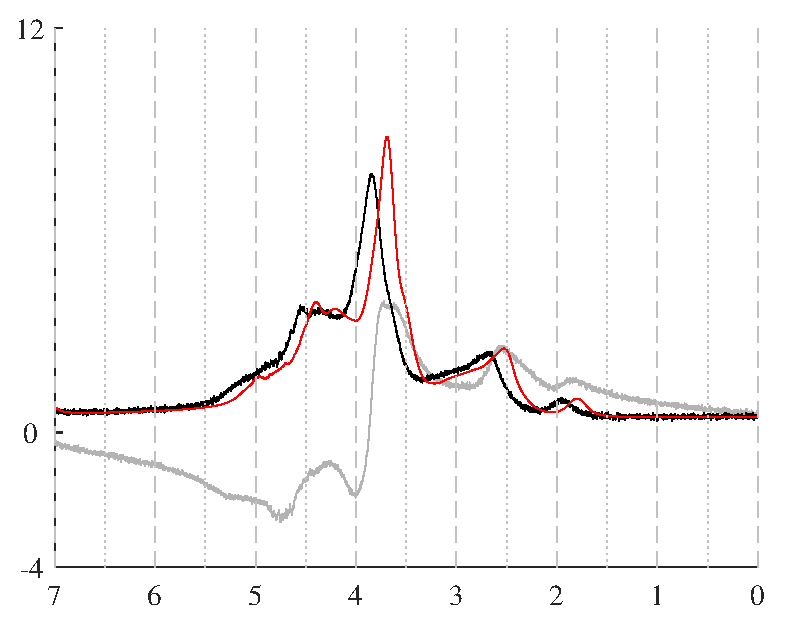
\includegraphics[width=0.93\textwidth,keepaspectratio]{images/30ms_B0_samples/30ms_curated_B0_sample_78Hz.eps}
    %     \vspace{3pt}
    % \end{subfigure}&%
    % \begin{subfigure}[c]{0.31\textwidth}
    %     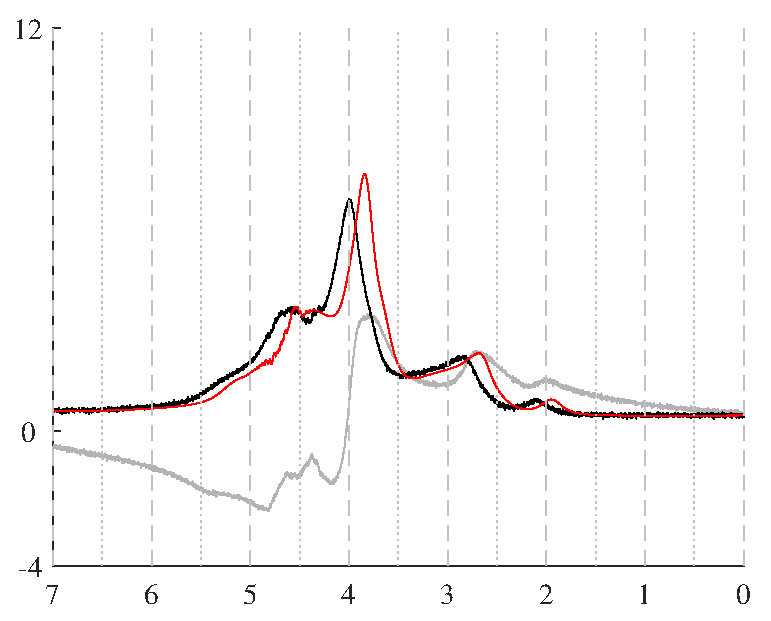
\includegraphics[width=0.93\textwidth,keepaspectratio]{images/30ms_B0_samples/30ms_curated_B0_sample_97Hz.eps}
    %     \vspace{3pt}
    % \end{subfigure}\\
    % \begin{subfigure}[c]{0.31\textwidth}
    %     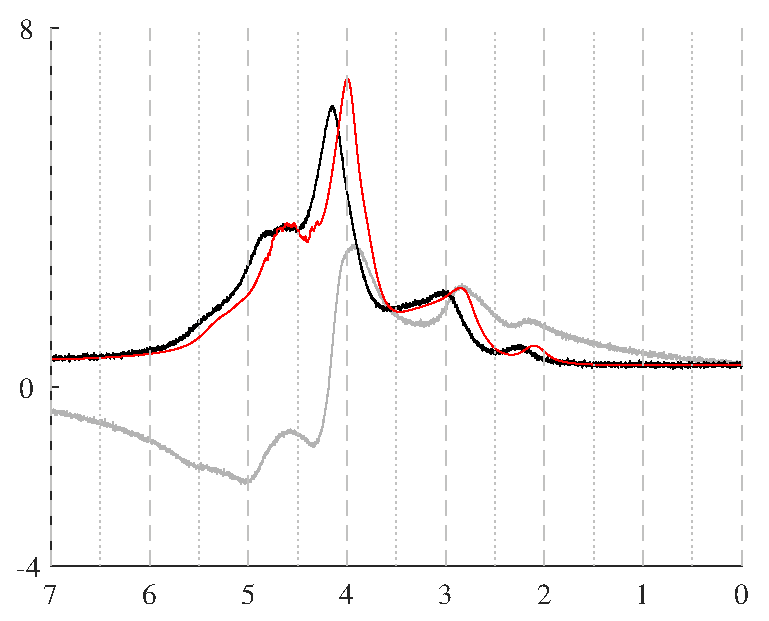
\includegraphics[width=0.93\textwidth,keepaspectratio]{images/30ms_B0_samples/30ms_curated_B0_sample_116Hz.eps}
    %     \vspace{3pt}
    % \end{subfigure}&
    % \begin{subfigure}[c]{0.31\textwidth}
    %     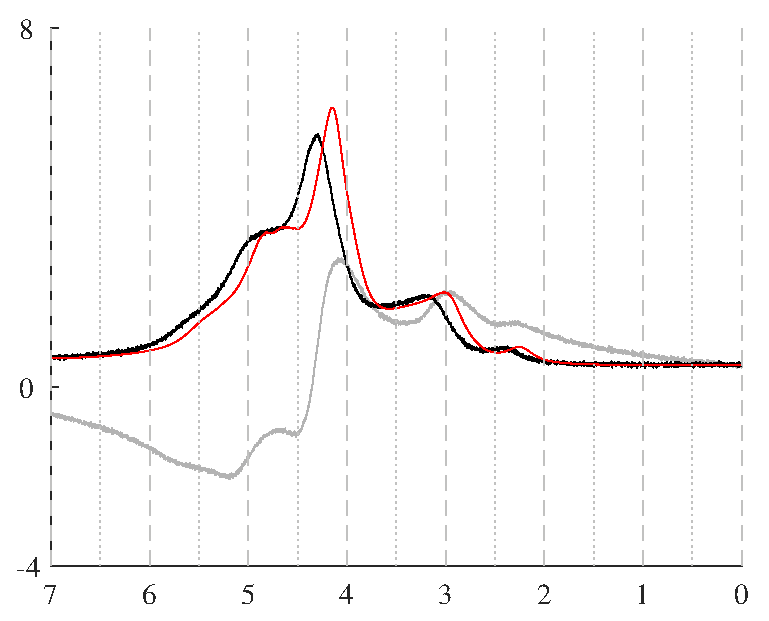
\includegraphics[width=0.93\textwidth,keepaspectratio]{images/30ms_B0_samples/30ms_curated_B0_sample_136Hz.eps}
    %     \vspace{3pt}
    % \end{subfigure}&
    % \begin{subfigure}[c]{0.31\textwidth}
    %     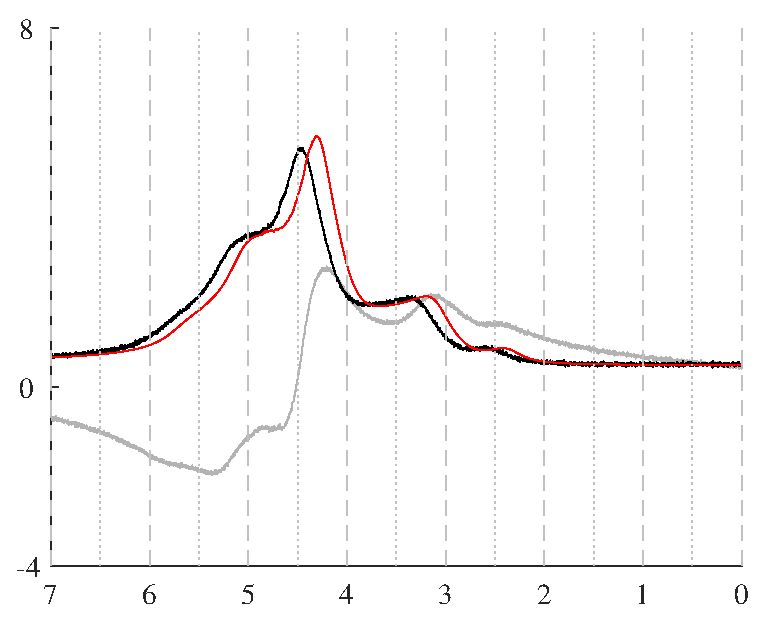
\includegraphics[width=0.93\textwidth,keepaspectratio]{images/30ms_B0_samples/30ms_curated_B0_sample_155Hz.eps}
    %     \vspace{3pt}
    % \end{subfigure}\\
    % \begin{subfigure}[c]{0.31\textwidth}
    %     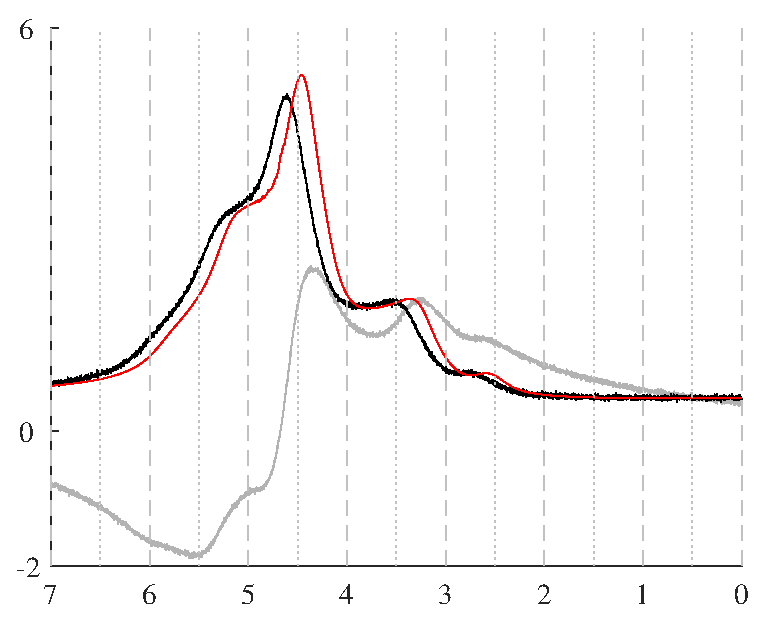
\includegraphics[width=0.93\textwidth,keepaspectratio]{images/30ms_B0_samples/30ms_curated_B0_sample_174Hz.eps}
    %     \vspace{3pt}
    % \end{subfigure}&
    % \begin{subfigure}[c]{0.31\textwidth}
    %     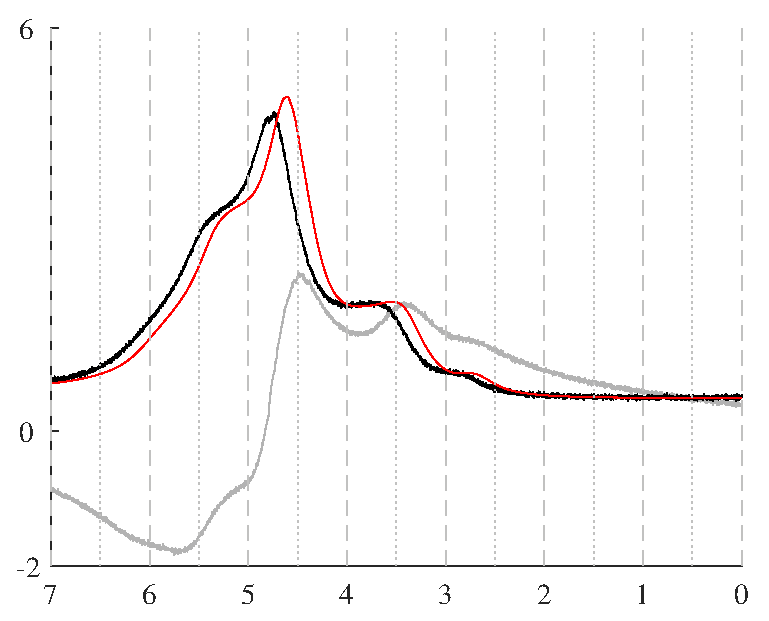
\includegraphics[width=0.93\textwidth,keepaspectratio]{images/30ms_B0_samples/30ms_curated_B0_sample_193Hz.eps}
    %     \vspace{3pt}
    % \end{subfigure}&%
    % \begin{subfigure}[c]{0.31\textwidth}
    %     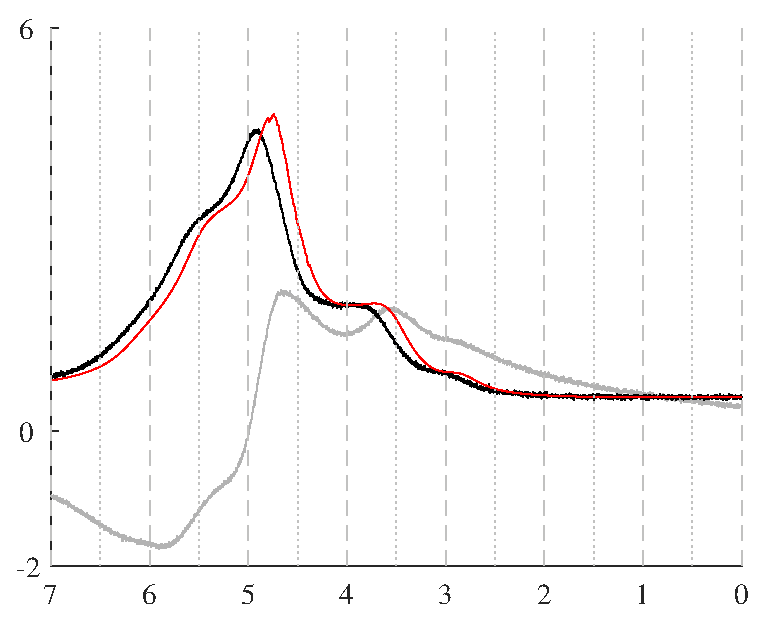
\includegraphics[width=0.93\textwidth,keepaspectratio]{images/30ms_B0_samples/30ms_curated_B0_sample_212Hz.eps}
    %     \vspace{3pt}
    % \end{subfigure}\\
    % \begin{subfigure}[c]{0.31\textwidth}
    %     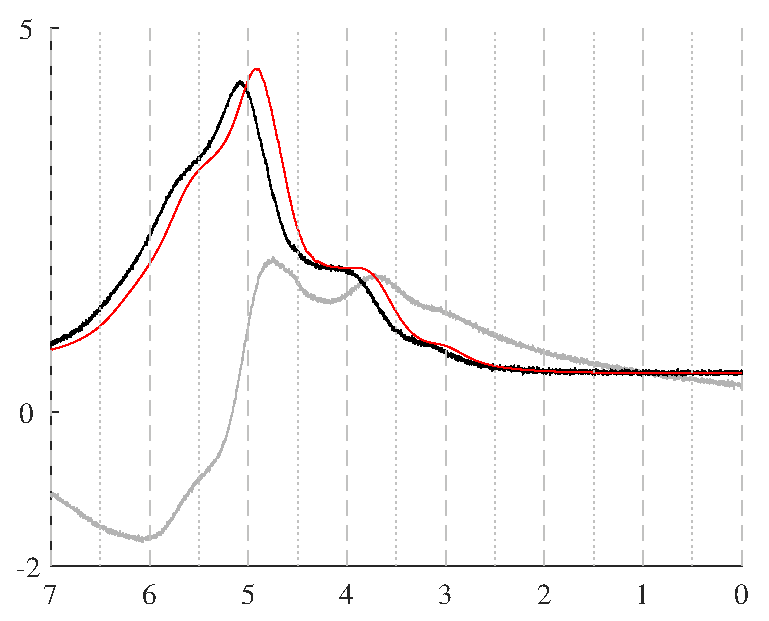
\includegraphics[width=0.93\textwidth,keepaspectratio]{images/30ms_B0_samples/30ms_curated_B0_sample_232Hz.eps}
    % \end{subfigure}&
    % \begin{subfigure}[c]{0.31\textwidth}
    %     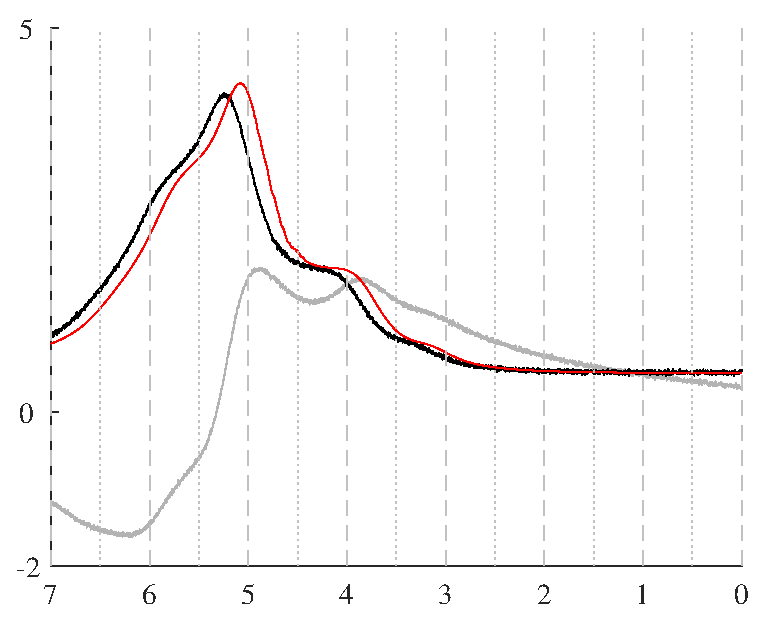
\includegraphics[width=0.93\textwidth,keepaspectratio]{images/30ms_B0_samples/30ms_curated_B0_sample_251Hz.eps}
    % \end{subfigure}&%
    % \begin{subfigure}[c]{0.31\textwidth}
    %     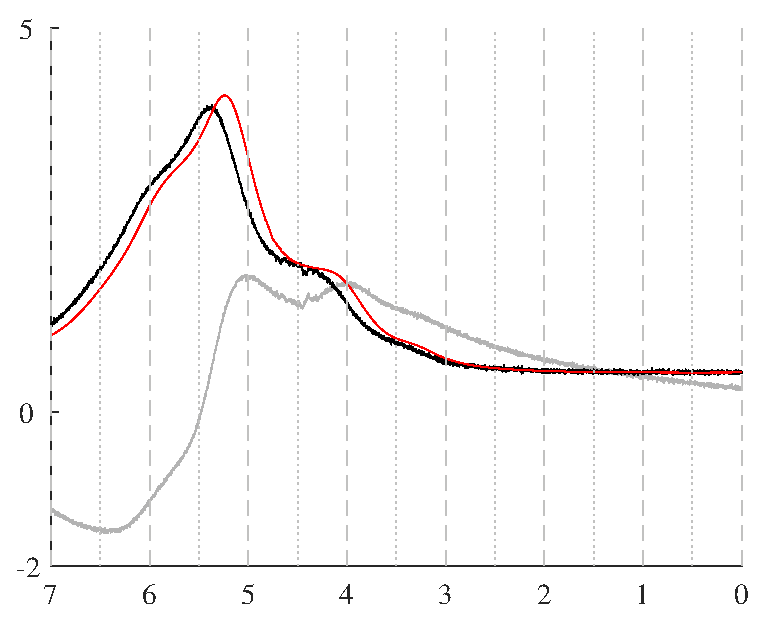
\includegraphics[width=0.93\textwidth,keepaspectratio]{images/30ms_B0_samples/30ms_curated_B0_sample_270Hz.eps}
    % \end{subfigure}
    % \end{tabular}
    \includegraphics[width=\textwidth,keepaspectratio]{images/compiled_figures/MRS_Sim_Figure_17_B0_inhomo_samples.png}
    \caption{Sample spectrum simulated for a PRESS sequence with TE=30ms that highlights the effect of $B_0$ inhomogeneities on the spectra. The mean inhomogeneities range from [1, 270] Hz and monotonically increase by 19Hz. As the inhomogeneities increase, the intensity of the spectra decreases, shown by the y-axis range, and causes a global frequency shift.}
    \label{fig:30ms B0 samples}
\end{figure}
